\section{Trusted Virtualization Platform}
The notion of a trusted visualized platform is coined by Trusted Computing Group's (TCG) companion architecture specification ``Virtualized Trusted Platform Architecture''~\cite{VTPA}. The TCG coined term and the architecture itself is rather vague but decisively extends the adjective \emph{trusted}, which should cause curiosity since intuitively only the TPM~\cite{ISOTPM} \emph{should} be trusted but not the entire platform. Recently, Akram et al.~\cite{digitaltrust} have adopted the term in a position paper on digital trust as their \emph{vision} for trusted cloud computing using the architecture in Fig. \ref{fig:vplatform}.
\begin{figure}[!ht]
  \centering
  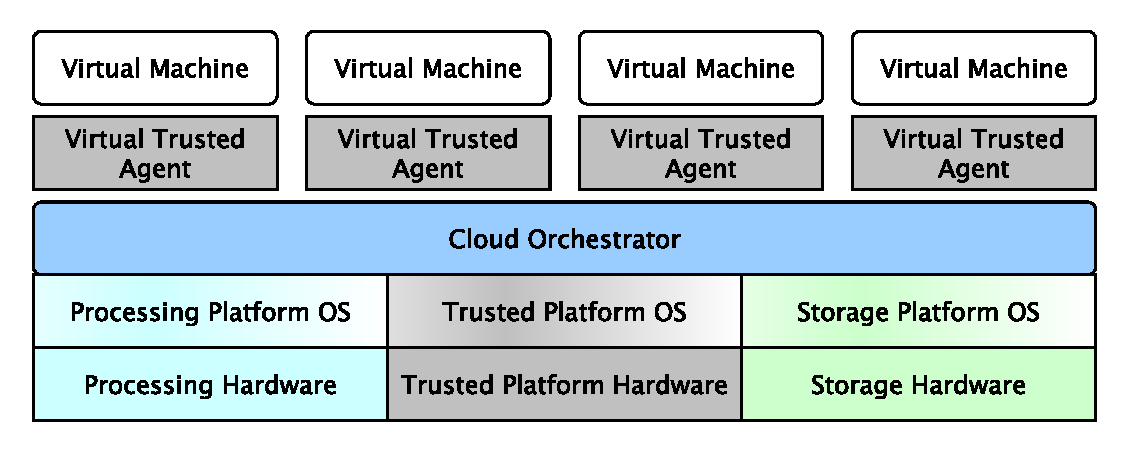
\includegraphics[scale=0.35]{figures/vplatform}
  \caption{Proposed architecture for Trusted Computing for Cloud Computing.~\cite{digitaltrust}}
  \label{fig:vplatform}
\end{figure}

While the concept of processing and storage hardware and a respective management (OS) is uncontroversial and not of general concern, the notion of Trusted Platform Hardware and a Trusted Platform OS raises questions, especially, in combination with Virtual Trusted Agents (represented by vTPMs).
Returning to the mathematicians' problem, it seems acceptable, even reasonable, that the Trusted Platform Hardware is in fact trustworthy and can be trusted. Specifications like \cite{ISOTPM} describe which functions and properties are required to synthesize a TPM. By inspecting a key credential, unique to each TPM, called Endorsement Key and a manufacture certificate, one can infer authenticity --- assuming the manufacturer is \emph{competent}.

\subsection{Levels of Trust and Specification}
The supposedly trusted platform OS seems to be a \emph{déjà vu} for our mathematician\cite{Dijkstra1979}: there are no indications about the trustworthiness other than that it carries the adjective \emph{trusted} from an external perspective. Described as quality of results, the mathematician upon interacting with the OS will need supporting evidence, or metadata other than the result itself to be convinced in every case that the interaction is correct or at least as desired or expected. This problem, although derived from an abstract case is quite intuitive: Unlike with the TPM, assuming trustworthiness of the OS is hardly justifiable. The reasons as to why that assumption is hard to substantiate are complex, especially since the specification is concerned with security. TCG's specification for Virtualized Trusted Platforms is considered a specification for \emph{TCG Applications}. It describes general requirements such as minimum required key sizes and lengths, it has a glossary of terms, and most importantly it describes interactions with virtualization layers, or hypervisors, such as the \emph{self-defending} Trusted Computing Base along with processes for instantiating, storing, or migrating virtual machines along with their \emph{Virtual Trust Agents}. The idea is that a \emph{vendor} can implement these requirements and refer to the conceived OS or platform as \emph{Trusted} Virtualization Platform. The problem here becomes apparent however, when the predicate \emph{trusted} derived from this specification is compared with the TPM itself: The Trusted OS along with Virtual Trusted Agents must be \emph{fully} specified and (remotely) verifiable\cite{sel4} to account for issues related to trusting software\cite{Lampson,Thompson}.


\subsection{Remote Attestation and Virtual Machines}
From an external perspective it seems unreasonable for a specification to suggest to a suspicious party that it should simply trust whoever claims to implement the specification. While this might seem reasonable from a perspective of contracts in business to business scenarios, the nature of IoT and the idea of plug and play invalidates such \emph{out-of-band} assurances. In order to be meaningful to a consumer or any interacting party, such a specification must provide a method to collect metadata about the potential trustee as to why it can be trusted within the scope of a specification. Defining a remote attestation process seems like a high priority task for any specification that builds on top of a TPM while requiring compliance of the implementer. Especially, since this compliance is easy to break in any software system if the potential trustee has malicious intent but also when the trustee is unaware of the fact that part of its software configuration are not suitable to an external party. The external party on the other hand would certainly like to see proof that its potential trustee implements the specification and has no additional or undesirable configuration on top of it. A focus on making a specification \emph{attestable} yields mutual benefits both for trustor and trustee.






